% Truth Probing Results: E1-E3 for Llama-3-8B-Instruct, Mistral-7B-Instruct-v0.3 and
% Qwen2.5-7B-Instruct. LaTeX version of the shared results doc.
% Compile from docs/:  latexmk -pdf truth_probing_results.tex
% Figures are read from ../results/comparison/ (scripts/compare_models.py).
\documentclass[11pt]{article}

\usepackage[T1]{fontenc}
\usepackage[utf8]{inputenc}
\usepackage[margin=2.5cm]{geometry}
\usepackage{amsmath}
\usepackage{booktabs}
\usepackage{graphicx}
\usepackage{enumitem}
\usepackage{url}
\usepackage[hidelinks]{hyperref}

\graphicspath{{../results/comparison/}}
\setlist{itemsep=2pt}
\setlength{\emergencystretch}{1em}
\newcommand{\topic}[1]{\texttt{#1}}
% table header cells, with \\ for a line break: \thead{...} centered, \thead[l]{...} left
\newcommand{\thead}[2][c]{\begin{tabular}[b]{@{}#1@{}}#2\end{tabular}}

\title{Truth Probing Results}
\author{ULLM project, group 11}
\date{14 October 2026}

\begin{document}
\maketitle

In all three models, truth becomes linearly decodable in the first third of the
network and plateaus at 0.97--0.98 pooled accuracy. It emerges at different depths per
topic (cities and translations first, facts last), and in Qwen about 0.1--0.15 relative
depth later than in Llama.

The direction is most shared across topics in the middle layers: a probe trained on one
topic reaches about 0.90 accuracy and 0.97 AUROC on the other five. In late layers,
transfer accuracy falls to 0.68--0.77 while AUROC stays at about 0.90. So the direction
stays mostly shared: in later layers each topic is mainly shifted along it, and only a
smaller part of the drop (AUROC $0.97 \rightarrow 0.90$) is a real change of direction.
Centering each topic at its own mean recovers 54--68\% of the late accuracy drop; the
rest is concentrated in facts and inventors.

\section{Setup}

E1--E3 ran exactly as Section~3.4 describes, on the 6,298 affirmative and negated
statements, at every layer of Llama-3-8B-Instruct (32 layers), Mistral-7B-Instruct-v0.3
(32) and Qwen2.5-7B-Instruct (28).

\begin{itemize}
  \item \textbf{Probe:} StandardScaler + L2 logistic regression, $C = 1$, lbfgs; all
        fits converged.
  \item \textbf{Folds:} 6-fold \texttt{StratifiedGroupKFold} (seed 0), built once per
        dataset; the fold file is byte-identical for all three models.
  \item \textbf{Depth:} layers $1, \dots, L$ are plotted at $\ell/L$. Layer 0 (the
        embedding) gives exactly 0.50 everywhere, as a sanity check, and is left out.
  \item \textbf{Files:} branch \path{topic-experiments}, folder
        \path{results/<model>/} (\path{e1_pooled.csv}, \path{e2_per_topic.csv},
        \path{e3_transfer.csv} with accuracy and AUROC, plus figures) and
        \path{results/comparison/} (three-model figures and
        \path{compare_summary.csv}). Code: \path{scripts/topic_probes.py},
        \path{scripts/compare_models.py}.
\end{itemize}

\section{E1: pooled baseline}

All three models reach the same plateau, but at different depths: Llama first, then
Mistral, then Qwen. The curve rises in the early-middle layers and stays flat to the
last layer, with a slight dip of at most 0.015 after the peak; the fold-to-fold standard
deviation is below 0.01 on the plateau (Table~\ref{tab:e1}, Figure~\ref{fig:e1}).

\begin{table}[ht]
  \centering
  \caption{Pooled probe (E1). Depths are relative depths $\ell/L$. All models are the
           instruction-tuned versions (Mistral: v0.3).}
  \label{tab:e1}
  \begin{tabular}{lcccc}
    \toprule
    \thead[l]{Model} & \thead{Depth,\\acc $\geq 0.75$} & \thead{Depth,\\acc $\geq 0.95$} & \thead{Peak\\accuracy} & \thead{Depth\\of peak} \\
    \midrule
    Llama-3-8B & 0.16 & 0.28 & 0.976 & 0.47 \\
    Mistral-7B & 0.19 & 0.34 & 0.969 & 0.47 \\
    Qwen2.5-7B & 0.25 & 0.46 & 0.976 & 0.64 \\
    \bottomrule
  \end{tabular}
\end{table}

\begin{figure}[ht]
  \centering
  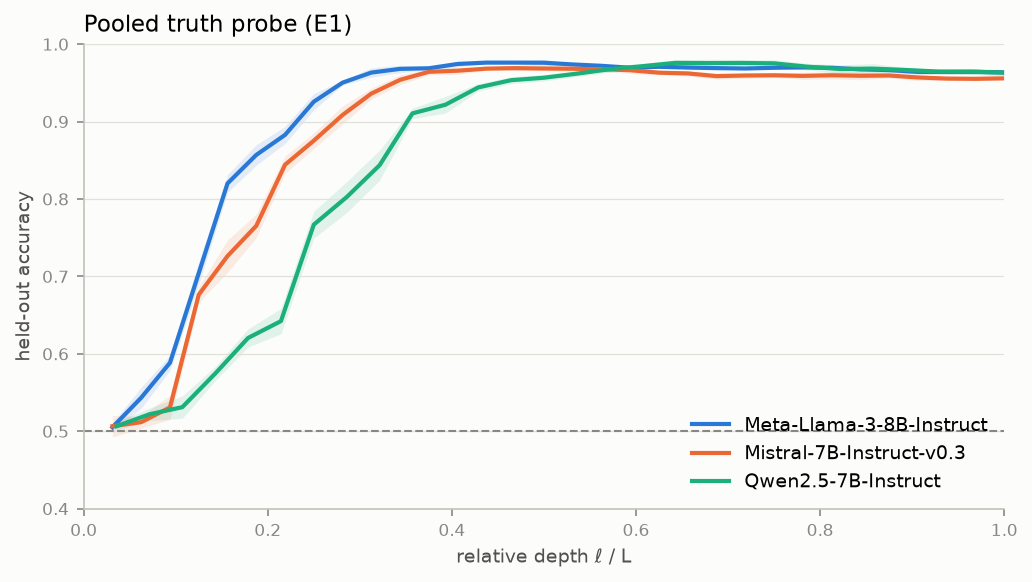
\includegraphics[width=0.7\linewidth]{compare_e1.png}
  \caption{Pooled held-out accuracy against relative depth for the three models.
           Shaded band: $\pm 1$ standard deviation over the six folds.}
  \label{fig:e1}
\end{figure}

\section{E2: per-topic depth profiles}

The depth at which truth emerges is not shared across topics, and the order of topics
is almost the same in all three models. Cities and Spanish--English translations cross
0.75 first. Facts cross it 0.15--0.19 relative depth later than cities, and inventors
sit in between.

Four topics plateau at 0.97--1.00. Inventors stay at about 0.94, and facts peak lowest
(0.89--0.92), then fall by 0.05--0.06 towards the last layer, the only topic that
clearly declines (Table~\ref{tab:e2}, Figure~\ref{fig:e2}).

\begin{table}[ht]
  \centering
  \caption{Per-topic probes (E2): first relative depth $\ell/L$ at which held-out
           accuracy reaches 0.75, with the highest held-out accuracy over all layers in
           parentheses. The 0.75 threshold is our choice and can be changed in
           \texttt{compare\_models.py}.}
  \label{tab:e2}
  \begin{tabular}{lccc}
    \toprule
    \thead[l]{Topic} & \thead{Llama} & \thead{Mistral} & \thead{Qwen} \\
    \midrule
    \topic{cities}       & 0.13 (0.999) & 0.13 (0.999) & 0.25 (0.998) \\
    \topic{sp\_en\_trans}  & 0.16 (1.000) & 0.16 (0.997) & 0.21 (1.000) \\
    \topic{animal\_class}  & 0.16 (0.994) & 0.22 (0.994) & 0.29 (0.994) \\
    \topic{element\_symb}  & 0.16 (1.000) & 0.22 (0.987) & 0.25 (0.997) \\
    \topic{inventors}    & 0.19 (0.943) & 0.25 (0.945) & 0.36 (0.949) \\
    \topic{facts}        & 0.28 (0.915) & 0.31 (0.885) & 0.43 (0.916) \\
    \bottomrule
  \end{tabular}
\end{table}

\begin{figure}[ht]
  \centering
  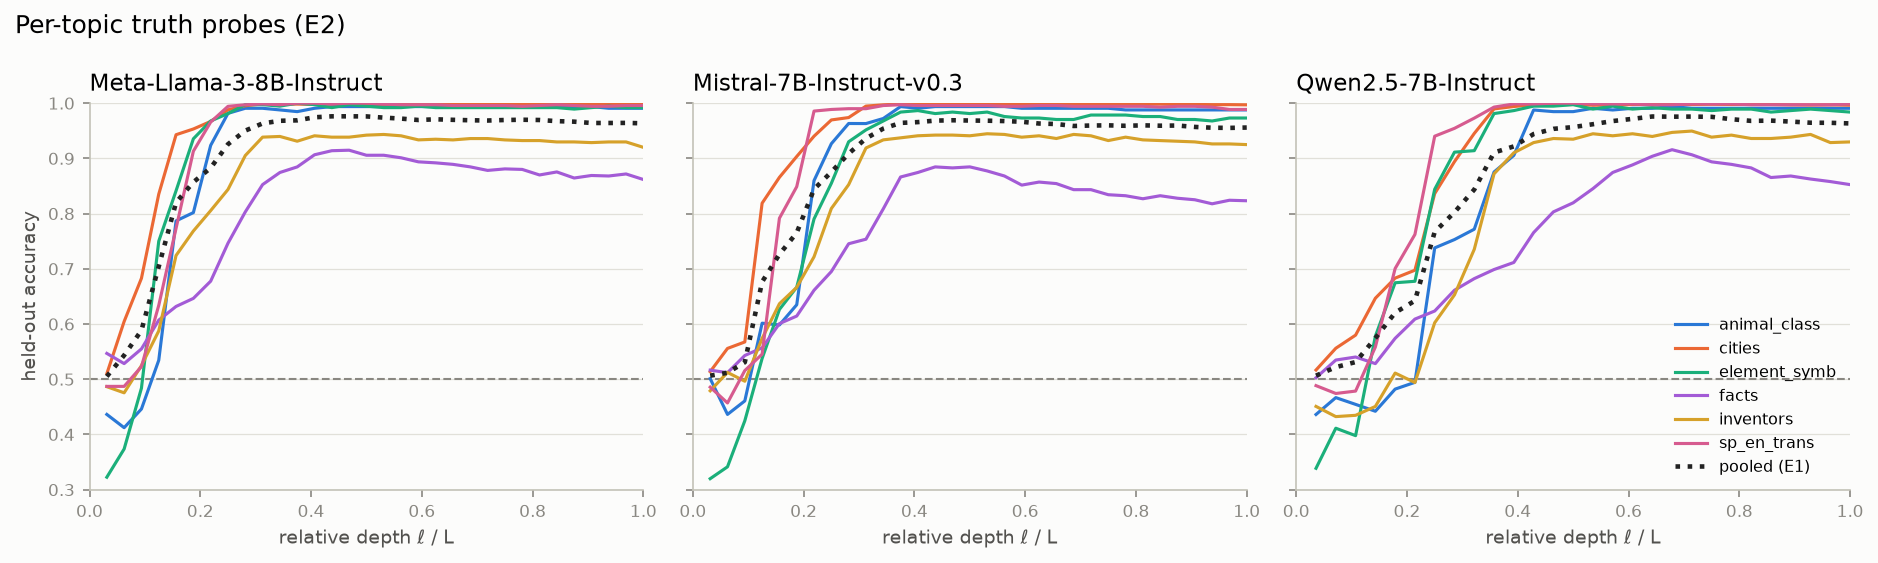
\includegraphics[width=\linewidth]{compare_e2.png}
  \caption{Per-topic held-out accuracy against relative depth, one panel per model.
           Dotted line: pooled probe (E1).}
  \label{fig:e2}
\end{figure}

\section{E3: cross-topic transfer}

A single truth direction is shared across topics in the middle of the network, at about
the same relative depth where E1 peaks. Transfer lags behind within-topic accuracy on
the way up, peaks at about 0.90 accuracy and 0.97 AUROC, and then declines, in accuracy
far more than in AUROC. The direction stays mostly shared; each topic mainly shifts
along it (Table~\ref{tab:e3}, Figure~\ref{fig:e3}).

\begin{table}[ht]
  \centering
  \caption{Cross-topic transfer (E3): means over the 30 off-diagonal entries of
           $A_\ell$. Within-topic (diagonal) accuracy stays at 0.95--0.96 to the last
           layer in all models.}
  \label{tab:e3}
  \begin{tabular}{lcccc}
    \toprule
    \thead[l]{Model} & \thead{Peak transfer\\acc (depth)} & \thead{AUROC at\\that depth} & \thead{Acc,\\last layer} & \thead{AUROC,\\last layer} \\
    \midrule
    Llama-3-8B & 0.914 (0.41) & 0.977 & 0.682 & 0.905 \\
    Mistral-7B & 0.892 (0.47) & 0.966 & 0.737 & 0.889 \\
    Qwen2.5-7B & 0.898 (0.68) & 0.977 & 0.770 & 0.910 \\
    \bottomrule
  \end{tabular}
\end{table}

\paragraph{Why late transfer drops.} The AUROC check of Section~3.4 answers this: from
the peak to the last layer, accuracy falls by 0.13--0.23, but AUROC only by about 0.07.
So most of the drop comes from topics being shifted along the probe direction, which
puts them on the wrong side of the threshold. The rest is a real change of direction,
concentrated in two topics:

\begin{itemize}
  \item \textbf{Facts and inventors are the hardest targets.} As test topics in the last
        layer they get AUROC 0.80--0.82 in all three models; the other four get
        0.85--0.99. Both topics are also the weakest within-topic (E2).
  \item \textbf{Element symbols and translations transfer worst as training topics by
        accuracy} (0.59--0.68 in the last layer), but their AUROC stays at 0.84--0.93:
        mostly an offset problem.
\end{itemize}

\paragraph{Topic-centered rerun.} Centering each topic at its own mean before training
and testing, as B\"urger et al.\ do, removes the offset between topics. It uses no
labels, and every topic is 50\% true. Transfer AUROC changes by at most 0.004, so only
accuracy moves (Table~\ref{tab:centered}, Figure~\ref{fig:centered}).

\begin{table}[ht]
  \centering
  \caption{Mean off-diagonal transfer accuracy without (raw) and with topic centering.
           Late drop recovered $=$ (centered $-$ raw accuracy at the last layer) $/$
           (raw peak $-$ raw last layer).}
  \label{tab:centered}
  \begin{tabular}{lccc}
    \toprule
    \thead[l]{Model} & \thead{Peak acc:\\raw $\rightarrow$ centered} & \thead{Last layer:\\raw $\rightarrow$ centered} & \thead{Late drop\\recovered} \\
    \midrule
    Llama-3-8B & $0.914 \rightarrow 0.944$ & $0.682 \rightarrow 0.839$ & 68\% \\
    Mistral-7B & $0.892 \rightarrow 0.922$ & $0.737 \rightarrow 0.820$ & 54\% \\
    Qwen2.5-7B & $0.898 \rightarrow 0.941$ & $0.770 \rightarrow 0.847$ & 60\% \\
    \bottomrule
  \end{tabular}
\end{table}

\begin{itemize}
  \item \textbf{The shift is the larger part.} Centering recovers 54--68\% of the
        late-layer accuracy drop, as the AUROC suggested.
  \item \textbf{A real change of direction remains.} Even centered, transfer falls by
        0.09--0.11 from its peak ($0.92$--$0.94 \rightarrow 0.82$--$0.85$), while
        within-topic accuracy stays at 0.95--0.96.
  \item \textbf{It is concentrated in facts and inventors.} As test topics in the last
        layer they reach 0.72--0.74 centered accuracy, against 0.77--0.96 for the other
        four.
\end{itemize}

\begin{figure}[ht]
  \centering
  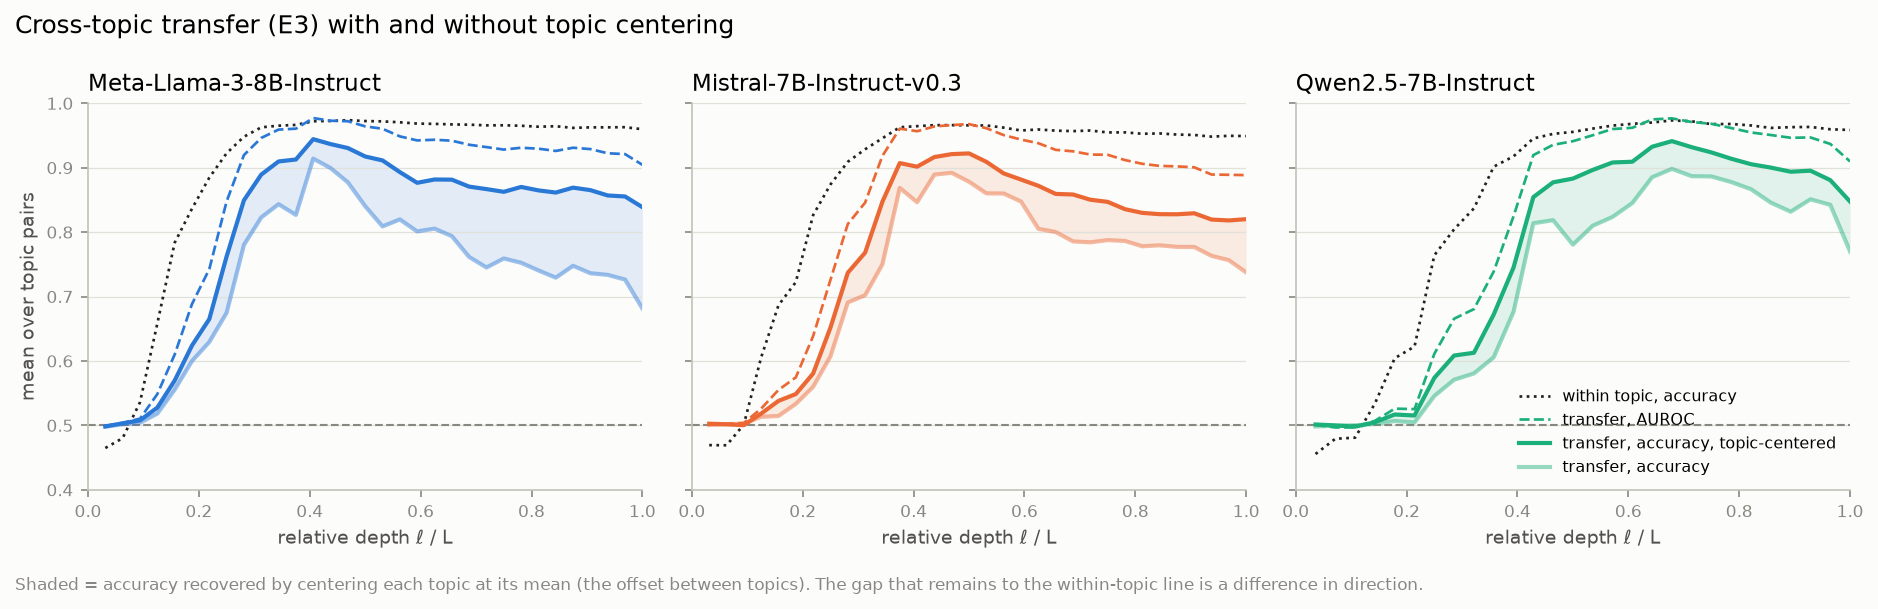
\includegraphics[width=\linewidth]{compare_e3_centering.png}
  \caption{Cross-topic transfer accuracy with and without topic centering, with
           transfer AUROC and within-topic accuracy, one panel per model. Shaded:
           accuracy recovered by centering each topic at its mean.}
  \label{fig:centered}
\end{figure}

\begin{figure}[ht]
  \centering
  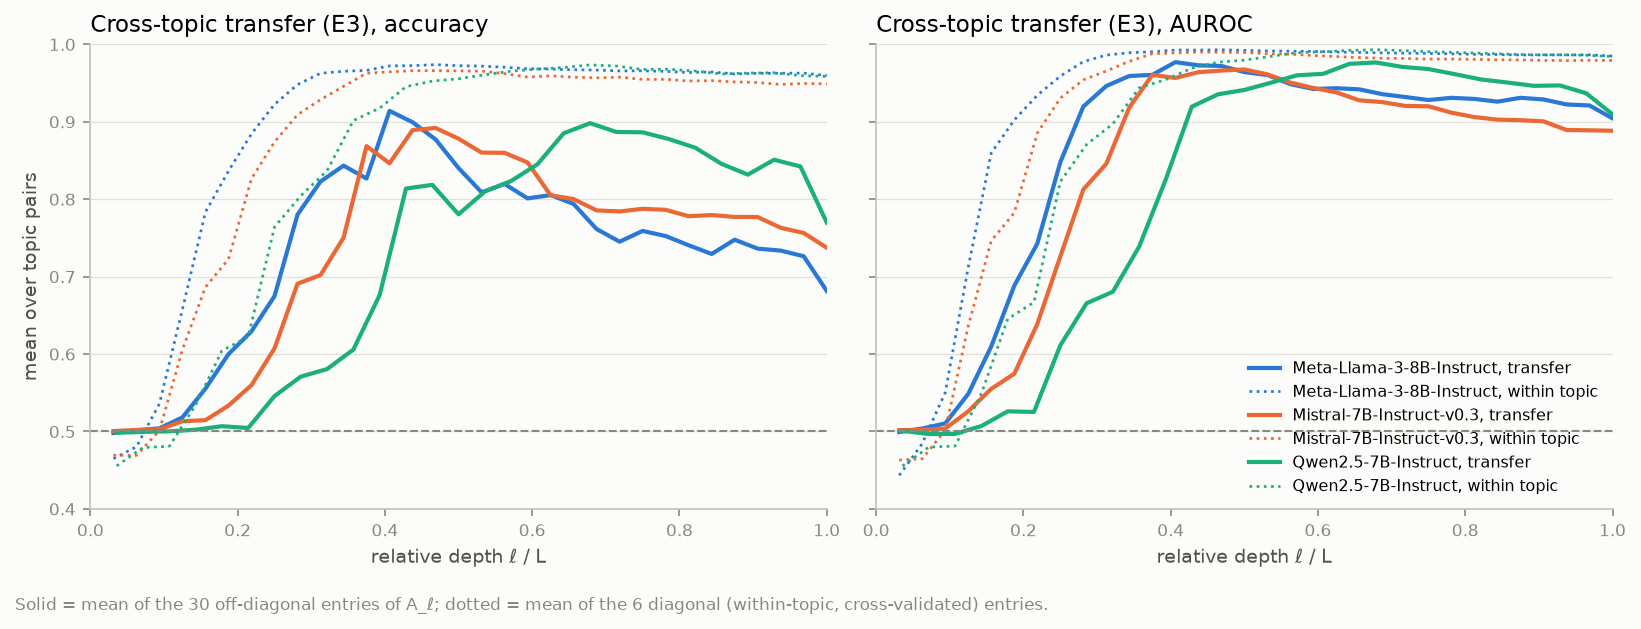
\includegraphics[width=\linewidth]{compare_e3.png}
  \caption{Mean cross-topic transfer accuracy (left) and AUROC (right) against relative
           depth. Solid: mean of the 30 off-diagonal entries of $A_\ell$; dotted: mean
           of the six diagonal (within-topic) entries.}
  \label{fig:e3}
\end{figure}

Full $6 \times 6$ matrices at 25/50/75/100\% depth: \texttt{results/<model>/e3\_matrices.png}.

\section{For Section 3 of the report}

Table~1 of the report can be filled in. Pooled with negations, every topic is balanced,
so chance is 50\% throughout (Table~\ref{tab:data}).

\begin{table}[ht]
  \centering
  \caption{Number of statements per topic after restricting to affirmative and negated
           statements. The share of true statements gives the chance level for each
           topic.}
  \label{tab:data}
  \begin{tabular}{lrrr}
    \toprule
    \thead[l]{Topic} & \thead{Affirm.} & \thead{Negated} & \thead{\% true} \\
    \midrule
    \topic{animal\_class} &   164 &   164 & 50.0 \\
    \topic{cities}       & 1,496 & 1,496 & 50.0 \\
    \topic{element\_symb} &   186 &   186 & 50.0 \\
    \topic{facts}        &   547 &   545 & 49.9 \\
    \topic{inventors}    &   406 &   406 & 50.0 \\
    \topic{sp\_en\_trans}  &   351 &   351 & 50.0 \\
    \midrule
    Total                & 3,150 & 3,148 & 50.0 \\
    \bottomrule
  \end{tabular}
\end{table}

Details the text does not state yet:

\begin{itemize}
  \item \textbf{Section 3.5:} we used $C = 1$ (lbfgs, max 5,000 iterations; every fit
        converged).
  \item \textbf{Section 3.2:} Mistral and Qwen ran in bfloat16, because Qwen2.5
        overflows in float16; Qwen activations were saved as float32. Llama ran and was
        saved in float16, with no overflowed values. Suggested sentence:
        ``LLaMA3-8B-Instruct was run in float16, Mistral-7B-Instruct-v0.3 and
        Qwen2.5-7B-Instruct in bfloat16, since Qwen2.5 overflows in float16.''
  \item \textbf{Section 4 footnote:} in layers 1--3, some topics score well below chance
        (\topic{element\_symb} about 0.32). This is a known artefact of cross-validation
        on features with no signal, not a finding.
\end{itemize}

\end{document}
